\documentclass[11pt]{article}
\usepackage[margin=1in]{geometry}
\usepackage[T1]{fontenc}
\usepackage{lmodern}
\usepackage{microtype}
\usepackage{graphicx}
\usepackage{booktabs}
\usepackage{amsmath}
\usepackage{url}
\usepackage[hidelinks]{hyperref}
\usepackage[numbers,sort&compress]{natbib}
\usepackage{xcolor}
\usepackage{caption}
\captionsetup{font=small,labelfont=bf}
\setlength{\parskip}{3pt}

\title{\textbf{GPU Canary: Border Inputs as a Two-Second Integrity Check for Silent Data Corruption in Deployed Language Models}}
\author{Rishva Tejan Iyer\\\small Independent researcher\\\small \texttt{rishtiyer@gmail.com}}
\date{October 29, 2026}

\begin{document}
\maketitle

\begin{abstract}
A GPU with a silent hardware fault returns wrong arithmetic without raising an error. Production studies report that such faults are routine at fleet scale, that three quarters of affected cards pass burn-in, and that vendor diagnostics recover about 70\% of them at several hours per card. The cheapest online check, redundant execution with bitwise comparison, is blind by construction to the common case of a unit that is wrong the same way on every run. We show that a language model already loaded on a GPU can act as its own integrity probe. We mine 64 \emph{border inputs}, prompts on which the model's top two next-token logits are nearly tied, so that any perturbation of the arithmetic flips the greedy decision, record their answers while the hardware is healthy, and later replay them and count mismatches. On an NVIDIA L4 in fp16 the reference is bit-stable across reruns, and a scan of 64 probes takes 2.5\,s. Against software-injected faults reproducing the patterns reported in production (a value zeroed, a sign flipped, a bit flipped, a relative bias of $10^{-3}$) at one corruption per hundred layer forwards, the probes flag 10 of 10 scans for every pattern, while 32 ordinary prompts flag between 0 and 8 of 10 and never see the $10^{-3}$ bias. Against persistent faults fixed at a random site, the probes flag 8 of 8 sites for every pattern on two models, redundant execution flags 0 of 8, and ordinary prompts 0 or 1 of 8. Under the RTL-derived permanent-fault model of LLM-PRISM, hard tensor-core defects are flagged at 15 of 16 sites by the probes, 1 of 16 by ordinary prompts, and 0 of 16 by redundant execution, while intermittent defects favour redundant execution; the two checks are complementary. The method is the border-input idea of recent model-change-detection work, redirected at the hardware. No genuinely defective GPU has been tested; all faults are injected, and we state the limits plainly.
\end{abstract}

\section{Introduction}

Large language models are served from fleets of accelerators, and accelerators fail quietly. A silent data corruption (SDC) is a wrong arithmetic result produced without any hardware error signal \citep{dixit2021sdc,hochschild2021cores}. Two production studies from ByteDance and its university collaborators, published this year, describe the problem for GPU training clusters in detail: 18 SDC incidents on 13 cards across 35 million GPU hours, incidents that cost training jobs worth millions of dollars, vendor diagnostics with roughly 70\% recall that occupy a card for eight hours or more, and generic stress tests that miss more than 60\% of defective devices \citep{lei2026aegis,zheng2026sdcwild}. Meta reports a hardware failure every 2.78 hours on a 16{,}000-GPU run, with about 1.4\% attributed to GPU SDC \citep{grattafiori2024llama3,altenbernd2026sdc}. The faults are not confined to new hardware: only a quarter were caught at burn-in, and 40\% appeared around one year into service \citep{zheng2026sdcwild}.

That literature is about training, where a detector can compare gradients, checksum collectives, or replay a step. Inference has no such hooks. A deployed model on a degraded card answers every request fluently, and nothing in its output says which card produced it. The one cheap online check available at inference, running the same input twice and comparing bitwise, cannot see a fault that is deterministic for a given input, and SDCHunter reports exactly such devices, with replay occurrence rates of 100\% and error magnitudes that escalate over time \citep{zheng2026sdcwild}.

This paper asks whether the model itself can be the detector. The observation we build on comes from a different community. When the top two next-token logits of a language model are almost tied, the greedy decision is decided by rounding, and so it changes with the dtype, kernel, or hardware that produced it. Zhang et al.\ used such border inputs to infer the serving platform \citep{zhang2024hspi}; Wimbauer et al.\ identified inference engine, attention backend, and GPU from prompt-response pairs \citep{wimbauer2026fingerprinting}; and Chauvin et al.\ (B3IT) used them to detect undisclosed model changes behind commercial APIs at a fraction of the cost of prior black-box methods \citep{chauvin2026b3it}. All three treat the hardware as a fixed property to be identified. We treat it as a quantity that drifts, and ask whether the same probes detect that drift when it is caused by a fault rather than a configuration change.

\paragraph{Contributions.}
(1) A health check for deployed GPUs that requires nothing but the model already loaded: 64 border probes, a saved reference, a 2.5\,s replay. (2) A measurement of its sensitivity against fault patterns taken from the production SDC literature and from RTL-derived permanent-fault signatures, on a real GPU in the dtype most inference runs in, with ordinary prompts as the control. (3) The observation that the check sees persistent faults that redundant execution cannot, and a scan budget analysis for intermittent faults. (4) A statement of what the evidence does not show.

\section{Background}

\paragraph{Silent data corruption in accelerators.}
Gate-level fault injection on a data-center GPU finds that NaN and infinity account for about 1\% of corrupted outputs, that nullification (a value replaced by zero) accounts for about half, and that single-bit flips are under 40\% of bit-flip events \citep{tung2026anatomy}. Production diagnosis finds faults to be data dependent and unit specific, intermittent at rates from 100\% of replays down to $10^{-6}$\% \citep{zheng2026sdcwild}, with one incident traced to a matmul that was wrong roughly twice per billion executions \citep{lei2026aegis}. Some defects manifest as value biases below $10^{-3}$ that later layers absorb \citep{zheng2026sdcwild}. We take our injected fault patterns from these descriptions.

\paragraph{Testing accelerators with chosen inputs.}
Using the workload itself to test the hardware is an established idea in the test community. Li et al.\ injected faults into DNN accelerator datapaths and proposed symptom-based detectors that watch the network's own outputs \citep{li2017errorprop}; Chaudhuri et al.\ survey functional test generation for systolic-array accelerators, where a small set of chosen inputs exercises the array and only functionally critical faults are targeted \citep{chaudhuri2023testing}. That work assumes a fixed network and access to the device under test. We inherit the premise and change the probe: a border input is a test pattern the language model supplies about itself, and the reference is the model's own earlier answer.

\paragraph{Border inputs.}
For a prompt $x$ with next-token logits $z(x)$, let $g(x) = z_{(1)} - z_{(2)}$ be the gap between the two largest logits. When $g$ is small relative to the rounding error of the arithmetic that produced $z$, the argmax is unstable under perturbation. HSPI selects such prompts and reads the platform from which token wins \citep{zhang2024hspi}; B3IT selects them to detect that the model behind an API has changed \citep{chauvin2026b3it}. Wimbauer et al.\ show the signal survives realistic deployment variation and conclude that removing it would require eliminating numerical differences between stacks \citep{wimbauer2026fingerprinting}. Our use is narrower: one stack, compared with itself over time.

\section{Method}

\paragraph{Probe mining.}
Given a model and its tokenizer, we score candidate prompts (a short list of ordinary sentences plus random windows of tokens) with one forward pass each in fp32 and keep the $n=64$ prompts with the smallest gap $g$ below a threshold (0.05 in logit units). The mined bank is specific to the model; a different model gets its own bank. Mining takes about a minute on a GPU.

\paragraph{Reference.}
On hardware believed healthy, run each probe once in the serving dtype and record the greedy token. The decode rule must be the one the serving path uses; we found that \texttt{topk} and \texttt{argmax} break exact ties differently, and that in bf16 18 of our 64 probes are exact ties, so a mismatched rule produces false drift. We use argmax on float32-cast logits, as the HuggingFace generation path does. The same applies to batch shape: common serving kernels are not batch-invariant, so the logits for one prompt depend on what else is in the batch \citep{he2025nondeterminism}. A reference recorded at one batch shape must be replayed at that shape, or the serving engine must use batch-invariant kernels; otherwise ordinary load variation reads as drift.

\paragraph{Scan.}
Replay the 64 probes, decode with the same rule, and count tokens that differ from the reference. Any mismatch is reported as drift together with the count. A scan is 64 single-token forwards: 2.5\,s for a 0.5B-parameter model on an L4 in fp16, with no batching.

\paragraph{Control.}
Everything is repeated with 32 ordinary prompts (complete sentences with a clear next token), so that the gain from choosing border inputs is measured rather than assumed.

\section{Experimental setup}

\paragraph{Hardware and models.}
NVIDIA L4 (driver 580, CUDA 12.9, PyTorch 2.9.1) on Google Cloud, and an AMD Ryzen 7 2700 CPU. Models: Qwen2.5-0.5B and Qwen2.5-1.5B \citep{qwen2025qwen25}, each with its own 64-probe bank mined on the L4. Serving dtype fp16 on the L4; fp32, fp16 and bf16 for the stability test; fp32 on the CPU.

\paragraph{Fault injection.}
We inject faults with forward hooks on \texttt{Linear} layers, so the model, weights, and kernels are untouched and only the activations leaving a layer are corrupted. Three fault models:
\begin{itemize}\itemsep1pt
\item \emph{Lane scale}: one output lane of one layer is multiplied by $1+\varepsilon$ on every forward, for $\varepsilon$ from $10^{-6}$ to $10^{2}$. A coarse sensitivity sweep.
\item \emph{Intermittent element}: with probability $r$ per \texttt{Linear} forward, one random output element is zeroed, sign-flipped, has one random bit of its float32 representation flipped, or is scaled by $1+10^{-3}$; $r\in\{1,0.1,0.01\}$. Position is random on every forward.
\item \emph{Persistent element}: one fixed element of one fixed layer is corrupted the same way on every forward (zero, sign, bias $10^{-3}$, bias $10^{-2}$), at 8 random sites per pattern. This models a stuck unit.
\item \emph{RTL-signature defects}: the permanent-fault model of LLM-PRISM \citep{tyagi2026prism}, whose error signatures come from RTL-level stuck-at simulation of an H100. A defect is pinned to one layer and one fixed output tile. Three unit types with the signatures the paper reports: a \emph{tensor core} defect corrupts a $3\times3$ patch of the output with the same bit flipped in every corrupted element; an \emph{FMA} defect produces sporadic high-magnitude outliers, here decided by the operand's low mantissa bits so that they are input-dependent but deterministic; an \emph{L1 cache} defect corrupts a whole output row with high-order bits flipped. Fault density 0.5 (the fixed fraction of the tile the defect touches), single-bit flips weighted 3:1 over double, and a per-forward rate $r\in\{1,0.1\}$ where $r=1$ is a hard stuck-at defect. 8 random sites per unit type and rate, on both models. Unit areas are not published; we ran all three types equally.
\end{itemize}

\paragraph{Metrics.}
For intermittent and persistent faults we report scan-level recall: the fraction of scans (or sites) on which at least one probe answer differed from the reference. For the persistent case we also run the standard redundant-execution check on the same 64 probes: run twice under the fault and compare bitwise. The ordinary-prompt control uses the same fault, the same scans, and its own clean reference computed in the same process.

\section{Results}

\paragraph{The reference is stable.}
Two independent runs of the bank on the L4 agreed on 64 of 64 probes in fp32, fp16 and bf16. On the CPU, 64 of 64 probes were stable across thread counts (1, 4, 8) and batched versus single execution. Across hardware, fp32 on the L4 matched fp32 on the Ryzen on 64 of 64 probes; fp16 differed on 4 and bf16 on 20 of 64. Dtype is the loud signal, hardware the quiet one, and neither moves on healthy hardware over time, which is what a drift detector needs.

\paragraph{Lane-scale sensitivity.}
Figure~\ref{fig:lane} shows the fraction of prompts whose answer changed as a function of the lane error. On the L4 in fp16 the first probe flips at $\varepsilon=10^{-2}$ (2 of 64) and 9 of 64 flip at $\varepsilon=1$; ordinary prompts show nothing until $\varepsilon=10$ (1 of 32). On the CPU in fp32 the probes need $\varepsilon=0.1$ for the first flip. Across both, border probes respond to a fault roughly one to two orders of magnitude smaller than ordinary prompts do.

\begin{figure}[t]\centering
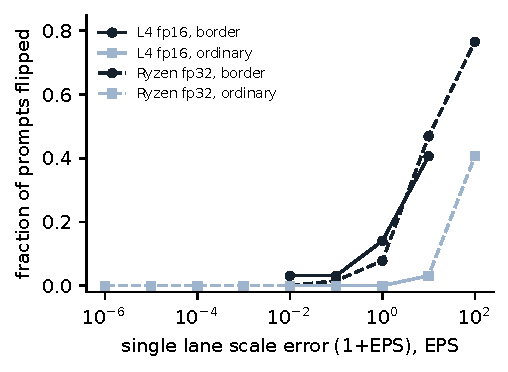
\includegraphics[width=0.55\linewidth]{figs/fig_lane.pdf}
\caption{Fraction of prompts whose greedy answer changed when one output lane of layer 20 is scaled by $1+\varepsilon$ on every forward. Qwen2.5-0.5B. Border probes (dark) respond at $\varepsilon=10^{-2}$ on the L4 in fp16; ordinary prompts (light) need $\varepsilon=10$.}
\label{fig:lane}
\end{figure}

\paragraph{Intermittent faults from the production patterns.}
Figure~\ref{fig:recall} and Table~\ref{tab:intermittent} give scan-level recall on the L4 in fp16. At one corruption per hundred \texttt{Linear} forwards, the probes flag 10 of 10 scans for every pattern. Ordinary prompts flag 0 of 10 for zeroing, sign flip and bias, and 8 of 10 for random bit flips, which are mostly large because exponent bits are included. The $10^{-3}$ bias, which SDCHunter singles out as the insidious case, is never seen by ordinary prompts at any rate and is flagged by the probes in 10 of 10 scans at $r=0.01$ and $r=0.1$. On the second model the three patterns tested at $r=0.01$ reproduce: 10 of 10 for the probes, 0, 2 and 0 of 10 for ordinary prompts.

\begin{figure}[t]\centering
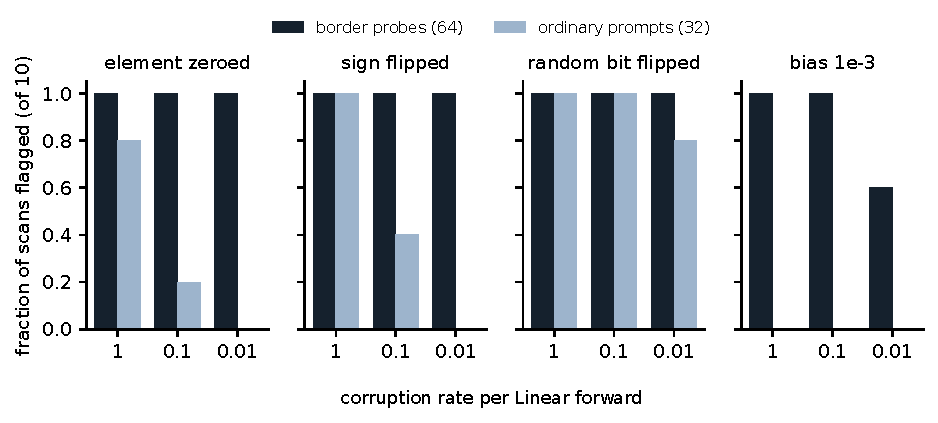
\includegraphics[width=\linewidth]{figs/fig_recall_l4.pdf}
\caption{Scan-level recall against intermittent element faults on the NVIDIA L4 in fp16, Qwen2.5-0.5B, ten full scans per bar. A scan is flagged if at least one answer differs from the reference.}
\label{fig:recall}
\end{figure}

\begin{table}[t]\centering\small
\caption{Intermittent faults, L4 fp16, Qwen2.5-0.5B. Scans flagged out of 10, border probes / ordinary prompts.}
\label{tab:intermittent}
\begin{tabular}{lccc}
\toprule
fault & $r=1$ & $r=0.1$ & $r=0.01$\\
\midrule
element zeroed & 10 / 8 & 10 / 2 & 10 / 0\\
sign flipped & 10 / 10 & 10 / 4 & 10 / 0\\
random bit flipped & 10 / 10 & 10 / 10 & 10 / 8\\
bias $10^{-3}$ & 10 / 0 & 10 / 0 & 10 / 0\\
\bottomrule
\end{tabular}
\end{table}

\paragraph{Persistent faults and redundant execution.}
Table~\ref{tab:persist} is the central result. For a unit that is wrong the same way on every forward, redundant execution reports agreement on 64 of 64 probes at every one of the 32 sites tested on each model, because both runs carry the same error; that blindness is by construction, and any check against a stored reference avoids it. The question is whether the stored answers move at all under a one-element fault, and here the choice of input decides: the border probes flag all 32 sites on both models, while ordinary prompts, with the same reference check, flag 1 of 32 and 0 of 32. The average number of probes that flipped per site, 10 for zeroing and 3 for the $10^{-3}$ bias on the 0.5B model, also gives a rough severity signal.

\begin{table}[t]\centering\small
\caption{Persistent element faults at 8 random sites per pattern. Sites flagged, border probes / ordinary prompts / redundant execution (run twice, compare).}
\label{tab:persist}
\begin{tabular}{lcc}
\toprule
pattern & Qwen2.5-0.5B & Qwen2.5-1.5B\\
\midrule
element zeroed & 8 / 1 / 0 & 8 / 0 / 0\\
sign flipped & 8 / 0 / 0 & 8 / 0 / 0\\
bias $10^{-3}$ & 8 / 0 / 0 & 8 / 0 / 0\\
bias $10^{-2}$ & 8 / 0 / 0 & 8 / 0 / 0\\
\bottomrule
\end{tabular}
\end{table}

\paragraph{Defects with RTL-derived signatures.}
Table~\ref{tab:prism} repeats the comparison under the LLM-PRISM fault model. For hard stuck-at defects ($r=1$) redundant execution flags 0 of 48 sites on the two models combined, as it must when both runs carry the same error. The border probes flag 47 of 48; ordinary prompts flag 23 of 48. The split by unit type is the informative part. FMA outliers and whole-row cache corruption are large faults and most ordinary prompts notice them too. The tensor-core signature, nine elements of one tile with one bit flipped, is the case that separates the methods: probes 15 of 16 sites, ordinary prompts 1 of 16, redundant execution 0 of 16. At $r=0.1$ the defect is intermittent and the picture inverts for the small faults: redundant execution, which compares two scans, flags 37 of 48 sites, while a single probe scan flags 31 of 48, and only 2 of 16 tensor-core sites. Intermittent small defects need repeated scans (Section 6); persistent ones need a reference. The two checks are complementary, and a deployment should run both.

\begin{table}[t]\centering\small
\caption{LLM-PRISM fault model, L4 fp16, 8 random sites per cell. Sites flagged, border probes / ordinary prompts / redundant execution.}
\label{tab:prism}
\begin{tabular}{llcc}
\toprule
unit signature & rate & Qwen2.5-0.5B & Qwen2.5-1.5B\\
\midrule
tensor core, $3\times3$ patch, same bit & 1.0 & 8 / 1 / 0 & 7 / 0 / 0\\
FMA, sporadic outliers & 1.0 & 8 / 8 / 0 & 8 / 8 / 0\\
L1 cache, whole row, high bits & 1.0 & 8 / 6 / 0 & 8 / 6 / 0\\
tensor core, $3\times3$ patch, same bit & 0.1 & 1 / 0 / 3 & 1 / 1 / 4\\
FMA, sporadic outliers & 0.1 & 8 / 7 / 8 & 8 / 5 / 8\\
L1 cache, whole row, high bits & 0.1 & 6 / 3 / 6 & 7 / 5 / 8\\
\bottomrule
\end{tabular}
\end{table}

\paragraph{fp32 on a CPU.}
Repeating the intermittent sweep in fp32 on the Ryzen reproduces the zero, sign and bit-flip rows but not the bias row: in fp32 a relative nudge of $10^{-3}$ on one element rarely reaches the argmax, and the probes flag it in 4 of 5 scans only at $r=1$ and never below. The bias sensitivity is therefore a property of half-precision serving, where most inference runs, not of the method in general.

\section{Scan budget for rare faults}

From the per-scan mismatch counts in the $r=0.01$ runs (ten scans per pattern, so a rough estimate) we take the probability $q$ that a single corruption flips at least one probe answer: $q\approx0.023$ for zeroing, $0.032$ for sign flips, $0.038$ for bit flips, and $0.007$ for the $10^{-3}$ bias. With $F=64\times168$ \texttt{Linear} forwards per scan of the 0.5B model, a fault firing at rate $r$ per forward is detected in one scan with probability $1-(1-q)^{Fr}$. Figure~\ref{fig:budget} converts this into the number of scans needed for 90\% detection. A fault at $r=10^{-3}$ is caught within 7 to 30 scans; at $r=10^{-4}$ within 70 to 300, which is one to five hours of hourly scans or minutes of continuous scanning; at $r=10^{-5}$ within a day of continuous 2.5\,s scans. The rarest production case, about $2\times10^{-9}$ per matmul \citep{lei2026aegis}, is out of reach of this and of any method that does not inspect every operation.

\begin{figure}[t]\centering
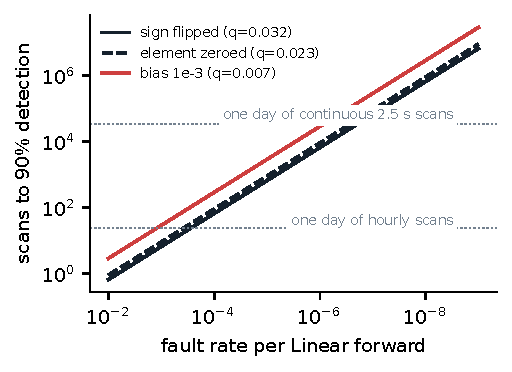
\includegraphics[width=0.55\linewidth]{figs/fig_budget.pdf}
\caption{Scans to 90\% detection as a function of fault rate, from the per-corruption flip probability $q$ measured at $r=0.01$. Dotted lines mark one day of hourly scans and one day of continuous scans.}
\label{fig:budget}
\end{figure}

\section{Limitations}

\begin{enumerate}\itemsep1pt
\item \textbf{No defective hardware was tested.} Every fault here is injected in software at the activation level. The patterns follow the production literature, but a real failing unit corrupts inside the kernel, with its own magnitudes and spatial structure. The LLM-PRISM signatures are the closest published description of real permanent faults, but we reconstructed them from the paper's text, not from its unreleased signature set, and we assigned equal weight to unit types whose silicon areas we do not know. The claim this paper supports is sensitivity to those patterns, not a recall figure on real faults.
\item \textbf{Sample sizes are small.} Ten scans per cell and eight sites per pattern. The results are consistent across two models and two machines, but confidence intervals are wide.
\item \textbf{One bank per model.} The probes are mined per model and would need re-mining after any model update; a model change and a hardware fault produce the same symptom, which is a feature for an integrity check and a confound for diagnosis.
\item \textbf{Exact ties.} In bf16 many border probes are exact ties whose outcome depends on the decode rule. A deployment must record the reference with the serving path's own decode, and any change to that path (engine, kernel, batch shape) is drift by this definition. Wimbauer et al.\ show such changes are detectable; whether they should be alarms is a policy question.
\item \textbf{Serving-engine stability is not measured.} The reference was shown stable across reruns of single, unbatched forwards in the HuggingFace path. Production engines batch dynamically and pick kernels by shape, and their outputs are known to vary with batch composition \citep{he2025nondeterminism}. We did not run the bank under vLLM or any serving engine. Until that is done, the false-alarm rate in a real deployment is unknown; the fix is either fixed-shape replay or batch-invariant kernels, both of which cost throughput.
\item \textbf{Small models.} Qwen2.5-0.5B and 1.5B. A single corrupted element is a larger fraction of the residual stream in these models than in a 70B model, and faults in deployment-scale models may be absorbed more often, or may hit more often per token because there are more forwards per token. We do not know the direction and did not test it.
\item \textbf{Rare faults.} Section 6 is a model, not a measurement, and it assumes corruptions are independent across forwards.
\item \textbf{Localization.} The count of flipped probes rises with severity, but we have not tried to infer which layer or unit is faulty from which probes flipped.
\end{enumerate}

\section{Related work}

Platform inference from outputs \citep{zhang2024hspi,wimbauer2026fingerprinting} and model-change detection \citep{chauvin2026b3it} are the direct ancestors of this method; they ask \emph{which} stack, we ask \emph{the same stack as yesterday}. Online SDC detection for training uses algorithmic checks on matmuls and deterministic redundant computation \citep{lei2026aegis,altenbernd2026sdc}, offline diagnosis replays production workloads to localize faulty devices \citep{zheng2026sdcwild}, and LLM-PRISM characterizes the training-time impact of permanent faults from RTL simulation \citep{tyagi2026prism}; we borrow its fault model for inference. These are stronger than our check wherever they apply, and they do not apply to a model serving requests. The accelerator-test literature uses chosen inputs and the network's own outputs to find faults \citep{li2017errorprop,chaudhuri2023testing}; our probes are that idea with the model choosing the inputs. Fleet-level CPU SDC studies \citep{dixit2021sdc,hochschild2021cores} established that the problem is systemic; the GPU error-pattern study of Tung et al.\ \citep{tung2026anatomy} supplied the fault distribution we injected.

\section{Conclusion}

A language model can check the arithmetic of the GPU it runs on, in the time of 64 single-token forwards, by answering questions it can barely decide and comparing with the day it was healthy. Against the fault patterns reported in production the check is sensitive where ordinary prompts are blind, and it sees persistent faults that redundant execution cannot. What remains is the one measurement that matters most and that we could not make: a genuinely defective card.

\section*{Reproducibility}
\begin{sloppypar}
Code, probe banks, reference signatures and every log behind each number are public at \url{https://github.com/rishvaiyer/gpu-canary}: \path{health/check.py}, \path{health/faultsim.py}, \path{health/persist.py} and \path{health/prism_fault.py}, with \path{probes/}, \path{refs/} and \path{data/}. Figures are regenerated from the logs by \path{paper/make_figures.py}. All GPU runs used a single rented L4 for under one hour in total.
\end{sloppypar}

\bibliographystyle{plainnat}
\bibliography{refs}
\end{document}
